\documentclass[11pt,letterpaper,boxed]{pset}

\usepackage[margin=0.75in]{geometry}
\usepackage{ulem}

\begin{document}

    \problemlist{PHYS051 HW02}
    \begin{center}
    	 Q27.3, P27.17, *E27.25, P27.4, P27.5, E29.29
    \end{center}
    
    \begin{problem} [Q27.3]
    	By analogy with $\Phi_E$, how would you define the flux $\Phi_g$ of a gravitational field? What is the flux of the Earth's gravitational field through the boundaries of a room, assumed to contain no matter? Through a spherical surface closely surrounding the Earth? Through a spherical surface the size of the Moon's orbit?
    \end{problem}
    \newpage
    
    \begin{problem} [P27.17]
    	A solid nonconducting sphere of radius $R$ carries a nonuniform charge distribution, with charge density $\rho=\rho_sr/R$, where $\rho_s$ is a constant and $r$ is the distance from the center of the sphere. Show that
    	
    	\begin{itemize}
    	    \item [(a)] the total charge on the sphere is $Q=\pi\rho_sR^3$ and
    	    \item [(b)] the electric field inside the sphere is given by $E=\frac{1}{4\pi\epsilon_0}\frac{Q}{R^4}r^2$.
    	    \item [(c)] What is the electric field outside the sphere ($r>R$)? You do not need to derive the result, simply explain why you know the answer.
    	\end{itemize}
    \end{problem}
    \newpage
    
    \begin{problem} [*E27.25]
    	Charge is distributed uniformly throughout an infinitely long cylinder of radius $R$.
    	
    	\begin{itemize}
    	    \item [(a)] Show that $E$ at a distance $r$ from the cylinder axis ($r< R$) is given by $E = \frac{\rho r}{2\epsilon_0}$, where $\rho$ is the volume charge density.
    	    \item [(b)] What result do you obtain for $r>R$?
    	\end{itemize}
    \end{problem}
    \newpage
    
    \begin{problem} [P27.4]
    	Figure 27-33 shows a charge $+q$ arranged as a uniform conducting sphere of radius $a$ and placed at the center of a spherical conducting shell of inner radius $b$ and outer radius $c$. The outer shell carries a charge of $-q$. Find $E(r)$ at locations
    	
    	\begin{itemize}
    	    \item [(a)] within the sphere $(r<a)$,
    	    \item [(b)] between the sphere and the shell $(a<r<b)$,
    	    \item [(c)] inside the shell $(b<r<c)$, and
    	    \item [(d)] outside the shell $(r>c)$.
    	    \item [(e)] What charges appear on the inner and outer surfaces of the shell?
    	\end{itemize}
    \end{problem}
    
    \begin{figure*} [ht]
        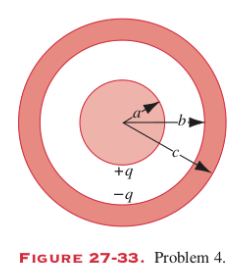
\includegraphics[width=125px]{HW2Images/P27-4.png}
        \label{fig:P27-4}
    \end{figure*}
    \newpage
    
    \begin{problem} [P27.5]
    	A very long conducting cylinder (length $L$) carrying a total charge $+q$ is surrounded by a conducting cylindrical shell (also of length $L$) with total charge $-2q$, as shown in cross section in Fig. 27-24. Use Gauss' law to find 
    	
    	
    	\begin{itemize}
    	    \item [(a)] the electric field at points outside the conducting shell,
    	    \item [(b)] the distribution of the charge on the conducting shell, and 
    	    \item [(c)] the electric field in the region between cylinders.
    	\end{itemize}
    \end{problem}
    
    \begin{figure*} [ht]
        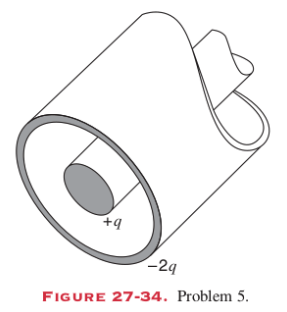
\includegraphics[width=125px]{HW2Images/P27-5.png}
        \label{fig:P27-5}
    \end{figure*}
    \newpage
    
    \begin{problem} [E29.29]
    	A 1-$\mu$C point charge is embedded in the center of a solid Pyrex sphere of radius $R$ = 10cm.
    	
    	\begin{itemize}
    	    \item [(a)] Calculate the electric field strength $E$ just beneath the surface of the sphere.
    	    \item [(b)] Assuming that there are no other \textit{free} charges, calculate the strength of the electric field just outside the surface of the sphere.
    	    \item [(c)] What is the induced surface charge density $\sigma_{ind}$ on the surface of the Pyrex sphere?
    	\end{itemize}
    \end{problem}
    \newpage
\end{document}